
%(BEGIN_QUESTION)
% Copyright 2011, Tony R. Kuphaldt, released under the Creative Commons Attribution License (v 1.0)
% This means you may do almost anything with this work of mine, so long as you give me proper credit

Examine this P\&ID and explain how a vacuum is produced in the sour water storage tank (V-10):

$$\includegraphics[width=15.5cm]{i0007rx01.eps}$$

Furthermore, identify what operators would have to do in order to halt the production of vacuum, to make it safe to open an access hatch on V-10 for inspection.  Also, identify how the level of sour water inside the tank is measured.

\vskip 20pt \vbox{\hrule \hbox{\strut \vrule{} {\bf Suggestions for Socratic discussion} \vrule} \hrule}

\begin{itemize}
\item{} Identify how this sour water storage tank is protected against excessive pressure or vacuum, which could rupture it or collapse it, respectively.
\end{itemize}

\underbar{file i03490}
%(END_QUESTION)





%(BEGIN_ANSWER)


%(END_ANSWER)





%(BEGIN_NOTES)

Vacuum is produced through the use of a {\it steam ejector}, where the throat of a venturi tube passing steam connects to the tank, sucking in vapors from the tank and into the steam flow.  

\vskip 10pt

In order to halt the production of vacuum, operators must halt the flow of steam through the ejector.  In order to safely secure vessel V-10 for inspection, one must secure all potential hazards including shutting the block valve between V-10 and the ejector to prevent steam and/or sour vapors from entering the vessel through that line.  

\vskip 10pt

The level instrument (LT-18) is a pressure-sensing instrument measuring the hydrostatic pressure at the bottom of the tank.  LG-19 is a tape-and-float instrument.









\filbreak \vskip 20pt \vbox{\hrule \hbox{\strut \vrule{} {\bf Virtual Troubleshooting} \vrule} \hrule}

\noindent
{\bf Predicting the effect of a given fault:} present each of the following faults to the students, one at a time, having them comment on all the effects each fault would produce.

\begin{itemize}
\item{} 
\item{} 
\item{} 
\end{itemize}


\vskip 10pt


\noindent
{\bf Identifying possible/impossible faults:} present symptoms to the students and then have them determine whether or not a series of suggested faults could account for all the symptoms, explaining {\it why} or {\it why not} for each proposed fault:

\begin{itemize}
\item{} Symptom: {\it FIC-27 shows flow at 15\% with setpoint at 60\% and output saturated at 100\%}
\item{} FT-27 failed low -- {\bf Yes}
\item{} FV-27 has insufficient air supply pressure -- {\bf Yes}, if valve is air-to-open
\item{} Heat exchanger E-2 shell-side clogged -- {\bf No}
\item{} Heat exchanger E-2 bypass valve left open -- {\bf No}
\item{} FV-27 bypass hand valve left open -- {\bf No}
\item{} Heat exchanger E-2 tube-side clogged -- {\bf Yes}
\item{} Pump P-102 shut off -- {\bf No}, if tank level is below the tower entry point
\item{} Water level in tank V-10 low -- {\bf Yes}, if it's so low that the pump is sucking air
\end{itemize}


\vskip 10pt


\noindent
{\bf Determining the utility of given diagnostic tests:} present symptoms to the students and then propose the following diagnostic tests one by one.  Students rate the value of each test, determining whether or not it would give useful information (i.e. tell us something we don't already know).  Students determine what different results for each test would indicate about the fault, if anything:

\begin{itemize}
\item{} Symptom: {\it }
\item{}  -- {\bf Yes/No}
\item{}  -- {\bf Yes/No}
\end{itemize}


\vskip 10pt


\noindent
{\bf Diagnosing a fault based on given symptoms:} imagine the ??? fails ??? in this system (don't reveal the fault to students!).  Present the operator's observation(s) to the students, have them consider possible faults and diagnostic strategies, and then tell them the results of tests they propose based on the following symptoms, until they have properly identified the nature and location of the fault:

\begin{itemize}
\item{} Operator observation: {\it }
\item{} 
\item{} 
\end{itemize}

%INDEX% Physics, dynamic fluids: venturi effect (steam ejector -- realistic P&ID shown)
%INDEX% Process: sour water stripping tower (realistic P&ID shown)

%(END_NOTES)


